\documentclass[onecolumn,10pt,cleanfoot]{asme2ej}

\usepackage{graphicx} %% for loading jpg figures
\usepackage{bm}
\usepackage{nicefrac}
\usepackage{mathtools}
\usepackage{amssymb}
\usepackage{amsmath}
\usepackage{parskip}
\usepackage{listings}
\usepackage{tablefootnote}
\usepackage{float}
\usepackage{xcolor}
\usepackage{xurl}
\usepackage{tikz}
\usepackage{caption}

\author{Grzegorz Kajda
    \affiliation{
	Bachelor Student, Robotics and Intelligent Systems\\ \\[-10pt]
	Department of Informatics The faculty of Mathematics and Natural Sciences\\ \\[-10pt]
    Email: grzegork@ifi.uio.no
    }
}


\begin{document}

\title{Simulating the Lipkin-Meshov-Glikov model on a classical computer}

\maketitle

\section{Abstract}

We present a comprehensive simulation of the simplified Hamiltonian of the Lipkin-Meshov-Glikov (LMG) model on a classical computer, employing the Variational Quantum Eigensolver (VQE) algorithm. Initially, we explore the outcomes arising from the application of diverse single qubit quantum gates to one qubit systems prepared in basis states. Subsequently, an entangler circuit is constructed, and one of the four bell pairs is prepared, to which we apply the Hadamard and CNOT gates. Utilizing our newfound grasp of the foundational principles governing quantum systems, we construct quantum circuits for generating ansatz states and methodically develop the VQE from ground up.

To assess the VQE's efficacy, we apply it to synthetic quantum systems representing single and two-particle systems, comparing its performance against numerical and analytical solvers. Transitioning to the Lipkin model, we leverage the properties of annihilation and creation operators to reformulate the Lipkin model's Hamiltonian first in terms of the quasi-spin operator and then Pauli operators. Employing this encoding scheme, we apply the VQE to systems with spin J=1 and 2, corresponding to Lipkin systems with two and four fermions, respectively. We compare the results against exact solutions obtained through standard diagonalization methods. This analysis provides valuable insights into the performance and accuracy of the VQE approach in tackling the Lipkin model's Hamiltonian.
	

\section{Introduction}
Since its emergence in the early 1900s, quantum mechanics has sparked fervent discussions among physicists, engaging luminaries of modern physics like Einstein, Dirac, Bohr, and many others. The discovery of the quantum realm profoundly reshaped our perspective and understanding of the world around us, unveiling a whole new realm of fundamental principles governing the very building blocks of the universe. With the advent of computer systems in the latter half of the 20th century, and the introduction of the quantum Turing machine in 1980, the field of quantum computing was born, ultimately leading to the construction of the first quantum computer in 1998. Recently, due to technological advances and discovery of new quantum algorithms, we have been granted to an extent, the capability of simulating simple many-body quantum models using classical computers.

An emerging research area in quantum computing focuses on the simulation of nuclear physics, leveraging the unique properties of quantum systems. Nuclear systems possess distinct characteristics that make them well-suited for exploration using quantum computers, providing insights into particle interactions. However, it is worth noting that quantum computers still face challenges, such as larger error rates compared to classical computers and vulnerability to noise, which can make working with them potentially difficult. Although the field of quantum computing is expanding rapidly, widespread accessibility remains limited, with companies like IBM offering only highly restricted access to their quantum technology. In light of these factors, we will employ a classical computer to simulate and analyze the simplified Lipkin-Meshkov-Glick model, showcasing the potential that quantum computing holds while acknowledging the current limitations in accessibility.

To facilitate our simulations, we will begin by constructing quantum circuits using single-qubit quantum gates. This approach will allow us to implement the Variational Quantum Eigensolver (VQE) algorithm effectively, enabling us to approximate the ground state energy of the Lipkin model for systems composed of two and four particles.

Apart from the introduction, this paper is organized into four sections. In Section Two, we will provide a comprehensive description of the theory and methods employed in this study. Following that, we will present our results, and finally, conclude with a summary of our findings.
 
 \section{\textbf{Section II: Theory and Method \\}}

 \subsection{Quantum gates}
The primary distinction between classical computers and their quantum counterparts lies in the nature of the data they process. In classical computing, the fundamental data unit is the binary digit, commonly known as a bit, which represents different voltage levels associated with low and high states. On the other hand, quantum computers utilize particles, such as atoms, as the information unitm leading to a fundamentally different approach to data handling. The unique properties of atoms and the underlying principles of quantum mechanics prevent us from treating them in the same manner as classical bits. For instance, in classical computing, logical gates like \textit{and}, \textit{or}, \textit{xor}, and \textit{nand} are commonly used for data processing, but these gates produce irreversible outcomes. However, on quantum computers, irreversible outcomes are generally not allowed, except in the case of measurement.

On a quantum computer, the fundamental data type used for storing information is the \textit{qubit}, which represents the digital manifestation of the wave function for a quantum particle. The principles of quantum mechanics dictate that the evolution of a quantum system can be mathematically described using unitary operators. This implies that the operations applied to quantum systems are inherently reversible. Consequently, at any given point in time, a quantum system can be fully characterized by a set of linear unitary operators. As a result, data processing on a quantum computer necessitates the use of reversible operators, enabling the "uncomputation" of the outcomes produced by quantum gates. The most basic of these operators are typically represented using 2x2 matrices. While these 2x2 operators quantum gates operate on individual qubits, by utilizing the Kronecker product (tensor product), we can in theory construct gates for quantum systems composed of arbitrary number of qubits. In practice we will often find ourselves restricted to at most 8 or 10 qubits before the computational overhead becomes too high.

The following are the basic quantum gates which we will utilize to contruct more complex gates and ciruits: 

\begin{enumerate}
	\item[\textbf{I}.] \textbf{Identity gate} \\
		This gate does nothing to the state of the qubit, as if a gate never was applied to the qubit in the first place.
		\begin{equation*}
			I = \begin{pmatrix}
			1 & 0 \\
			0 & 1 \\
		\end{pmatrix}.
	\end{equation*}

	\item[\textbf{II.}] \textbf{Pauli-X gate} \\
		The Pauli-X gate, also known as the quantum NOT-gate, flips the probability amplitudes $\alpha$ and $\beta$, meaning that these values swap place in the state vector. 
		\begin{equation*}
			X = \begin{pmatrix}
			0 & 1 \\
			1 & 0 \\
		\end{pmatrix}.
	\end{equation*}

	\item[\textbf{III.}] \textbf{Pauli-Y gate} \\
		The action of the Pauli Y gate can be described as the mapping of $|0>$ to $i|1>$ and $|1>$ to $i¦0>$. The action of the gate can also be viewed as a rotation of the state of the qubit around the y-axis of the Bloch sphere by 180 degrees.
		\begin{equation*}
			Y = \begin{pmatrix}
			0 & -i \\
			i & 0 \\
		\end{pmatrix}.
	\end{equation*}

	\item[\textbf{IV.}] \textbf{Pauli-Z gate} \\
		The Pauli Z gate flips the phase of $|1>$ to $-|1>$ while leaving $|0>$, meaning it flips the relative phase of the qubit. 
		\begin{equation*}
			Z = \begin{pmatrix}
			1 & 0 \\
			0 & -1 \\
		\end{pmatrix}.
	\end{equation*}

	\item[\textbf{V.}] \textbf{Hadamard gate} \\
		The result of applying the Hadamard gate to either $|0>$ or $|1>$ is a qubit in a super position of both states, with both the basis states having a 50\% of occuring. The result is the exactly the same, independent of which of the basis states the qubit is prepared in.
		\begin{equation*}
			H = \frac{1}{\sqrt{2}} \begin{pmatrix}
			1 & 1 \\
			1 & -1 \\
		\end{pmatrix}.
	\end{equation*}

	\item[\textbf{VI.}] \textbf{Phase gate} \\
		The Phase gate, when applied to a qubit, represent the rotation of the second part of a qubit state vector corresponding to $|1>$ by 90 degrees around the z-axis of the bloch sphere.

		\begin{equation*}
			S = \begin{pmatrix}
			1 & 0 \\
			0 & i \\
		\end{pmatrix}.
	\end{equation*}
		For a single qubit, application of each of these matrices represents a rotation of the qubit on the \textit{Bloch sphere (Fig. 1)}. (For more details, take a look at [Hundt, p.56] or [Nielsen, p.19])

\begin{figure}[ht]
  \centering
  \includegraphics[width=0.3\textwidth]{Bloch_sphere.svg.png}
  \caption{Caption text describing the picture.}
  \label{fig:example}
\end{figure}

	\item[\textbf{VII.}] \textbf{CNOT-gate} \\
		The Controlled-NOT gate, often abbreviated as CNOT, is a more complex gate that combines the Identity and Pauli-X gates using a Kronecker product. This gate is designed to operate on quantum systems composed of two qubits rather than a single qubit. The name of the gate provides a clue about its functionality. By using the first qubit as a control signal, the CNOT gate flips the amplitudes of the second qubit if the control qubit is in the basis state |1>, which corresponds to an active high signal in classical computing. However, if the control qubit is in the state |0>, no changes are applied to the second qubit. The specific gate we are discussing here is the $CNOT_{0,1}$-gate, where the first qubit serves as the control signal.
		It's important to note that we can also use the second qubit as the control signal by simply changing the order of the gates in the tensor product used to create the CNOT gate from $I \otimes X$ to $X \otimes I$. In matrix form, this operator is represented by a 4x4 matrix that can be written as:
		
		\begin{equation*}
		 CNOT_{0,1} = \begin{pmatrix}
			1 & 0 & 0 & 0 \\
			0 & 1 & 0 & 0 \\
			0 & 0 & 0 & 1 \\
			0 & 0 & 1 & 0 \\
		\end{pmatrix}
	\end{equation*}

\end{enumerate}



\subsection{Lipkin-Meshkov-Glick model}
The Lipkin-Meshkov-Glick (LMG) model, often called Lipkin model, is a quantum model describing the collective beahvior of a large number of particles which was introduced in 1964 for the purpose of studying approximation methods used to solve many-body problems. Since its introuduction, it has become one of the standard benchmarks [Physical review C] for many-body methods in nuclear and particle physics. The model describes a system of N fermions (i.e. particles with half-integer spin values like electrons and quarks) which are distributed among two energy levels with quantum numbers $\sigma$ = ±1. The upper level has $2\sigma$ = +1 and energy $e_{1}$ = $e/2$, while the lower level has $2\sigma$ = -1 and energy $e_{2}$ = $e/2$. This can be visualized in the following way

\begin{figure}[H]
	\centering
	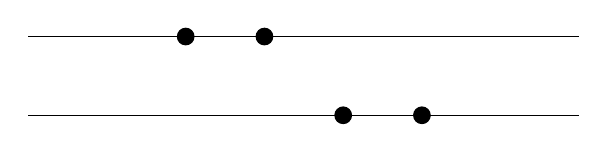
\begin{tikzpicture}
	  % Draw the parallel lines
	  \draw (0,0) -- (7,0);
	  \draw (0,1) -- (7,1);
	  
	  % Draw the small circles on the lines
	  \foreach \x in {2,3}
	  {
		\filldraw (\x,1) circle (3pt);

	  }
	  \foreach \x in {4,5}
	  {
		\filldraw (\x,0) circle (3pt);
	  }
	\end{tikzpicture}
	\caption{Figure showing the distrubution of four fermions among two energy levels}
\end{figure}

The figure depicts two horizontal lines representing the mentioned distinct energy levels, while the dots on the lines represent four fermions that in this case are evenly distributed between these levels. Each fermion in the figure corresponds to its own substate, characterized by quantum numbers $p = 1, 2, 3, 4$. It is important to note that in the figure, each particle occupies its own unique state. This behavior is typical of fermions, which obey the \textit{Pauli exclusion principle} [Basdevant, p. 348], meaning that two independent fermions cannot occupy the same state at exactly the same time (Do no dwelve on this too much, this is simply the nature of reality sorrounding us).

Now the Lipkin model is described through its Hamiltonian, a matrix correpsonds to the total energy of a physicial and is fundamental plays a fundamental role in the describing the evolution of a quantum system. Here, the Hamiltonian of the system is given by 
\begin{equation}
\hat{H} = \hat{H}_{0} + \hat{H}_{1} + \hat{H}_{2}.
\end{equation}

where each of the the $\hat{H}_{i}$ can be written in terms of the creation and annihilation operators

\begin{equation}
\hat{H}_0 = \frac{1}{2}\varepsilon\sum_{\sigma,p}\sigma a_{\sigma,p}^{\dagger}a_{\sigma,p},
\end{equation}

\begin{equation}
\hat{H}_1 = \frac{1}{2}V\sum_{\sigma,p,p'} a_{\sigma,p}^{\dagger}a_{\sigma,p'}^{\dagger}a_{-\sigma,p'}a_{-\sigma,p},
\end{equation}

\begin{equation}
\hat{H}_2 = \frac{1}{2}W\sum_{\sigma,p,p'} a_{\sigma,p}^{\dagger}a_{-\sigma,p'}^{\dagger}a_{\sigma,p'}a_{-\sigma,p}.
\end{equation}

Where \textit{V} and \textit{W} are constants, $\hat{H}_1$ represents the interaction that can move pairs of fermions between the energy levels, while $\hat{H}_2$ corresponds to the spin-exchange term, scattering one particle up and one down. These operators are in turn expressed in term of creation and annihilation operators, whose role in the context of a quantum mechanical many-body model, is the manipulation of the number of particles in specific substates. For instance, applying a creation operator to the upper energy level in Fig. 1 would increase the number of fermions in that energy level by one. One notable property of these operators is their ability to express the Hamiltonian of the Lipkin model in terms of the so-called \textit{quasi-spin operators} and the \textit{number operator}, where the former display behavior analogous to that of spin operators. Defining the quasi-spin operators in terms of creation and annihilation operators leads to the following equivalences 

\begin{equation}
\hat{J}_{+} = \sum_{p} a_{p+}^{\dagger}a_{p-},
\end{equation}

\begin{equation}
\hat{J}_{-} = \sum_{p} a_{p-}^{\dagger}a_{p+},
\end{equation}

\begin{equation}
\hat{J}_{z} = \frac{1}{2}\sum_{p\sigma} \sigma a_{p\sigma}^{\dagger}a_{p\sigma}, 
\end{equation}

\begin{equation}
\hat{J}^{2} = J_{+}J_{-} + J_{z}^{2} - J_{z}.
\end{equation}

which when substituted into the equation for the Hamiltonian $\hat{H}$ , the equation for \textit{N=2} particles is given by

\begin{equation}
	H_I = 2\sum_{p}\hat{J}_z(p) - \frac{V}{2}\sum_{p \neq q}(\hat{J}_+(p)\hat{J}_+(q) + \hat{J}_-(q)\hat{J}_-(p)) - \frac{W}{2}\sum_{p \neq q}(\hat{J}_+(p)\hat{J}_-(q) - \hat{J}_-(p)\hat{J}_+(q))
\end{equation}

Since the quasi-spin operators exhibit behavior similar to regular spin operators, they follow the commutation relations of angular momentum (for a detailed proof, refer to [Fys5429, lecture notes week 8]). This property is of great importance because fermions, such as electrons, are particles with half-integer spin (1/2-spin). It means that a fermion possesses intrinsic spin on its own (independent of its motion) [Basdevant, p.275]. In the context of atomic systems, the energy eigenstates are intimately connected to spin [Nielsen, p.310]. Therefore, when describing a system composed of atomic particles, it is crucial to consider these internal degrees of freedom.

By utilizing quasi-spin operators, we can account for these internal degrees of freedom and incorporate them into our calculations. This allows us to rewrite the Hamiltonian of the Lipkin model in a more convenient form. Consequently, we can express the Hamiltonian matrix in terms of the Pauli operators mentioned in the previous subsection. This transformation facilitates the analysis and study of the Lipkin model, providing insights into its energy levels and dynamics. Before proceeding however, we are going to simplify the Hamiltonian slightly more by setting the spin-exchange term equal to zero, resulting in a dimensionless Hamiltonian
\begin{equation}
\hat{H} = \epsilon\hat{J}_z - \frac{1}{2}V(\hat{J}_+\hat{J}_+ + \hat{J}_-\hat{J}_-).
\end{equation}

Having established the fundamental understanding of our problem and model, we move onto the encoding scheme we will apply to equation (10) for the case of the total spin \textit{J=1,2}, corresponding to situations when the model consists of \textit{N=2,4} particles.

\subsection{Encoding in terms of Pauli matrices}
As we happend to mention above, the quasi-spin operators in the expression for Hamiltonian of the Lipkin model presented in \textit{equation (10)} can be rewritten in terms of the pauli matrices. Using the definitions of the quasi-spin $\hat{J}$ presented in [Basdevant, p.233] and [Fys5419, week8] 

\begin{equation}
\begin{aligned}
	\hat{J}_x^{(n)} &\rightarrow \frac{X_n}{2}, \\
	\hat{J}_y^{(n)} &\rightarrow \frac{Y_n}{2}, \\
	\hat{J}_z^{(n)} &\rightarrow \frac{Z_n}{2}, 
\end{aligned}
\end{equation}

where \textit{X, Y} and \textit{Z} are the 2x2 Pauli operators. Having done that, we still need to express the ladder operators in terms of these new mappings

\begin{equation}
J_{\pm} = J_x \pm iJ_y
\end{equation}. 

With all the necessary definitions in place, rewriting the Hamiltonian in terms of Pauli matrices becomes a straightforward task. We can substitute the appropriate terms into Equation (10) and combine the resulting operators using the Kronecker product. For the Hamiltonian with N=2, the Hamiltonian matrix can be expressed as the sum of the following tensor products:

\begin{equation}
H = \frac{1}{2} (Z_0 \otimes I + I \otimes Z_1) - \frac{v}{2} (X_1 \otimes X_2 - Y_1 \otimes Y_2), 
\end{equation}


The reason we are interested in rewriting the Hamiltonian a second time is because of how measurements are performed on quantum computers for particle systems. Our goal is to measure the states of the particles in basis states |0⟩ and |1⟩ (or combinations of these states). These basis states correspond to the north and south poles of the Bloch sphere (as shown in Figure 1), and interestingly, they are also the eigenstates of the Pauli Z matrix. This means that measurements are typically performed along the Z-axis. Therefore, in order to perform measurements, we need to express the Lipkin model in terms of the Pauli operators and then rotate the Hamiltonian into the Z-basis using gate equivalences.

\subsection{Analytical method: Diagonalization}
In solving the Lipkin model, we employ the eigendecomposition technique to find exact solutions by diagonalizing the Hamiltonian matrix. This technique relies on the fundamental property that self-adjoint operators, including the Hamiltonian, can be diagonalized. This implies the existence of orthogonal eigenvectors denoted by $\mathbf{v}$ and corresponding eigenvalues denoted by $\lambda$, satisfying the equation $\mathbf{A} \mathbf{v} = \lambda \mathbf{v}$.

Since the Hamiltonian is a Hermitian operator [Scherer, p.38], which is self-adjoint, we can apply the eigendecomposition technique to it. By solving the characteristic equation $\det(H - \epsilon I) = 0$, where $H$ represents the Hamiltonian matrix and $I$ is the identity matrix, we can determine all the eigenvalues of the Hamiltonian. These eigenvalues represent the possible energy states within the Lipkin model.

The eigendecomposition method serves as a powerful tool for obtaining precise solutions to the Lipkin model and gaining insights into its energy spectrum. By diagonalizing the Hamiltonian matrix, we can extract valuable information regarding the system's energy levels and associated eigenvectors, which describe the various states of the system.


\subsection{Power iteration}
In our endeavor to showcase the prowess of the variational quantum algorithm, we will employ the power method for finding an approximate solution to the problem of finding the ground state of the Hamiltonian. However, we will tailor it slightly to seek the lowest eigenvalue instead of the largest. This method is remarkably straightforward, involving the computation of a matrix-vector product between our target matrix and a randomly initialized vector. The resulting product is then assigned to a new vector, which is subsequently normalized. This iterative process is repeated for a specified number of iterations or until convergence is attained.

The key insight of the power method is that with each multiplication, the initially initialized vector aligns itself more closely with the eigenvector corresponding to the lowest eigenvalue of the target matrix. Convergence is determined by measuring the absolute value of the difference between the product of the current and previous iterations of the algorithm.

By employing the power method with the necessary modifications, we can effectively find the lowest eigenvalue and its corresponding eigenvector, thereby gaining valuable insights into the properties and behavior of the matrix of interest. A detailed descripton of the method is presented in [Chapla, p.794].


\subsection{Variational Quantum Eigensolver}
The Variational Quantum Eigensolver (VQE) is a method used to estimate the ground state energy of a given Hamiltonian, such as the Lipkin Hamiltonian. This algorithm is specifically designed to handle Hamiltonian matrices that can be expressed as a sum of a polynomial number of terms involving Pauli operators [Hundt, p.242]. Examples of such Hamiltonians include the Lipkin model, Ising model, and the Harmonic Oscillator.

To estimate the ground state energy, the VQE algorithm involves three stages. In the first stage, an ansatz state is created, which is an initial state parameterized and constructed using single-qubit rotation matrices, namely $R_x$ and $R_y$. These rotations correspond to rotations around the x- and y-axes of the Bloch sphere shown in Figure 1. If the system consists of multiple qubits, entanglement is introduced among the qubits of the ansatz state using Controlled-NOT gates. This is done due to the unknown level of entanglement between the qubits of the system prior to performing measurements.

In the second stage of the algorithm, measurements are performed on the system state according to \textit{Postulate 3} for quantum measurements presented in [Nielsen, p.84-85]. During measurement, the qubit (or the wave function simulated using a qubit) collapses into one of the possible states of the system. This process is repeated a large number of times, and the resulting observations are used to approximate the probabilities associated with each possible substate of the system. Since the measurements are performed using a classical computer, it becomes easier to perform a large number of measurements and achieve accurate approximations of the probability amplitudes without the need to physically prepare particles for the system. As a result, efficient computation of the probabilities is enabled. 

The last and final stage of the VQE algorithm is focused on finding the optimal parameters for our ansatz in order to minimize the expectation value produced by the algorithm. The parameters we aim to tune are the angles $\theta$ and $\phi$ corresponding to the rotations around the x- and y-axes of the Bloch sphere. A naive approach would involve incrementally iterating through a large number of angles to obtain a precise approximation of the ground state energy over time. However, this approach becomes inefficient for larger many-body systems with dozens of particles. Hundt proposes the use of gradient descent as a more effective method for approximating the optimal angles for our ansatz [Hundt, p. 247]. Fortunately, we can easily define the gradient of our parameterized ansatz. The expectation value can be measured in terms of the ansatz as follows:


\begin{equation}
\langle \psi \vert \hat{H} \vert \psi \rangle = \langle 0 \vert R_i(\phi)^{\dagger} \hat{H} R_i(\phi) \vert 0 \rangle.
\end{equation}. 

If we for instance derivate with respect to the angle $\phi$, we arrive at 

\begin{equation}
\frac{\partial}{\partial \phi} \left[\langle \psi(\theta,\phi) \vert \boldsymbol{H} \vert \psi(\theta,\phi) \rangle\right] = \langle \psi(\theta,\phi) \vert \boldsymbol{H} \left(-\frac{\imath}{2} \boldsymbol{\sigma}_y \vert \psi(\theta,\phi) \rangle + \mathrm{h.c.}\right)
\end{equation}. 

Following the methodology presented in [Fys5419, week11], we arrive at a final expression for the derivative of the expectation value

\begin{equation}
\langle \psi \vert \boldsymbol{I}^{\dagger}\hat{H}\left(-\frac{\imath}{2}\boldsymbol{\sigma}_i\vert \psi \rangle\right) = \frac{1}{2}\left[\langle \psi \vert R_i\left(\frac{\pi}{2}\right)^{\dagger}\hat{H}R_i\left(\frac{\pi}{2}\right)\vert \psi \rangle - \langle \psi \vert R_i\left(-\frac{\pi}{2}\right)^{\dagger}\hat{H}R_i\left(-\frac{\pi}{2}\right)^{\dagger}\vert \psi \rangle\right] = \frac{1}{2}\left(\langle\hat{H}(\phi+\frac{\pi}{2})\rangle - \langle\hat{H}(\phi-\frac{\pi}{2})\rangle\right).
\end{equation}. 

We will perform measurements and use the following gradient to tune our parameters to arrive at the final value.

\section{Section III: Results}

With the theory and methods explained, we can now present the results achieved by simulating the quanatum gates and variational quantum eigensolver.

\subsection{Application of quantum gates to single qubits basis states}

As the first step of our project, we prepared single qubits in their basis state $|0>$ and $|1>$ and studied the result the application of the various quantum gates had on these one qubit systems. The effect each gate had on the basis states is presented below in the order the gates were listed in \textbf{Section II}. The results of applying the gates are: 

		\begin{enumerate}
			\item[\textbf{I}. ] Identity gate \\
				The result of applying both the $\sigma_0$ gate to both $|0>$ and $|1>$ results in the exact same states, as the identity gate is simply the identity matrix. Presented using matrices and vectors, the results can be written.
				\[
				I \begin{pmatrix}
				\alpha \\
				\beta
				\end{pmatrix}
				=
				\begin{pmatrix}
				1 & 0 \\
				0 & 1
				\end{pmatrix} \\ \\ \\
				\begin{pmatrix}
				\alpha \\
				\beta
				\end{pmatrix}
				=
				\begin{pmatrix}
				\alpha \\
				\beta
				\end{pmatrix}
				\]
			\item[\textbf{II}. ] Pauli-X gate \\
				The application of the Pauli X gate result in flipping of the probability amplitudes of the qubit, resulting in $\alpha$ and $\beta$ swapping places in the qubit. 
				\[
				I \begin{pmatrix}
				\alpha \\
				\beta
				\end{pmatrix}
				=
				\begin{pmatrix}
				0 & 1 \\
				1 & 0
				\end{pmatrix} \\ \\ \\
				\begin{pmatrix}
				\alpha \\
				\beta
				\end{pmatrix}
				=
				\begin{pmatrix}
				\beta \\
				\alpha
				\end{pmatrix}
				\] 
			\item[\textbf{III}. ] Pauli-Y gate \\
				The application of the Y-gate resulted in the exact behavipur described in point III of \textbf{Section II: Quantum gates}, a rotation of the qubits amplitudes bu 180 degrees around the y-axis. The result presented as a matrix-vector product is: 
				\[
				Y \begin{pmatrix}
				\alpha \\
				\beta
				\end{pmatrix}
				=
				\begin{pmatrix}
				0 & -i \\
				i & 0
				\end{pmatrix}
				\begin{pmatrix}
				\alpha \\
				\beta
				\end{pmatrix}
				=
				\begin{pmatrix}
				-i\beta \\
				i\alpha
				\end{pmatrix}
				\] 	
			\item[\textbf{VI}. ] Pauli-Z gate \\
				Just as expected based on the description provieded in the theory part, the Z-gate flips the relative phase of the state vector of our qubit. The result visualized using matrix-vector product is
				\[
				Z \begin{pmatrix}
				\alpha \\
				\beta
				\end{pmatrix}
				=
				\begin{pmatrix}
				1 & 0 \\
				0 & -1
				\end{pmatrix}
				\begin{pmatrix}
				\alpha \\
				\beta
				\end{pmatrix}
				=
				\begin{pmatrix}
				\alpha \\
				-\beta
				\end{pmatrix}
				\]
			\item[\textbf{VI}. ] Pauli-Z gate \\





			

		\end{enumerate}


\end{document}


